% Options for packages loaded elsewhere
\PassOptionsToPackage{unicode}{hyperref}
\PassOptionsToPackage{hyphens}{url}
%
\documentclass[
  a4paper,
  portrait]{book}

\usepackage{amsmath,amssymb}
\usepackage{iftex}
\ifPDFTeX
  \usepackage[T1]{fontenc}
  \usepackage[utf8]{inputenc}
  \usepackage{textcomp} % provide euro and other symbols
\else % if luatex or xetex
  \usepackage{unicode-math}
  \defaultfontfeatures{Scale=MatchLowercase}
  \defaultfontfeatures[\rmfamily]{Ligatures=TeX,Scale=1}
\fi
\usepackage{lmodern}
\ifPDFTeX\else  
    % xetex/luatex font selection
\fi
% Use upquote if available, for straight quotes in verbatim environments
\IfFileExists{upquote.sty}{\usepackage{upquote}}{}
\IfFileExists{microtype.sty}{% use microtype if available
  \usepackage[]{microtype}
  \UseMicrotypeSet[protrusion]{basicmath} % disable protrusion for tt fonts
}{}
\makeatletter
\@ifundefined{KOMAClassName}{% if non-KOMA class
  \IfFileExists{parskip.sty}{%
    \usepackage{parskip}
  }{% else
    \setlength{\parindent}{0pt}
    \setlength{\parskip}{6pt plus 2pt minus 1pt}}
}{% if KOMA class
  \KOMAoptions{parskip=half}}
\makeatother
\usepackage{xcolor}
\setlength{\emergencystretch}{3em} % prevent overfull lines
\setcounter{secnumdepth}{5}
% Make \paragraph and \subparagraph free-standing
\makeatletter
\ifx\paragraph\undefined\else
  \let\oldparagraph\paragraph
  \renewcommand{\paragraph}{
    \@ifstar
      \xxxParagraphStar
      \xxxParagraphNoStar
  }
  \newcommand{\xxxParagraphStar}[1]{\oldparagraph*{#1}\mbox{}}
  \newcommand{\xxxParagraphNoStar}[1]{\oldparagraph{#1}\mbox{}}
\fi
\ifx\subparagraph\undefined\else
  \let\oldsubparagraph\subparagraph
  \renewcommand{\subparagraph}{
    \@ifstar
      \xxxSubParagraphStar
      \xxxSubParagraphNoStar
  }
  \newcommand{\xxxSubParagraphStar}[1]{\oldsubparagraph*{#1}\mbox{}}
  \newcommand{\xxxSubParagraphNoStar}[1]{\oldsubparagraph{#1}\mbox{}}
\fi
\makeatother

\usepackage{color}
\usepackage{fancyvrb}
\newcommand{\VerbBar}{|}
\newcommand{\VERB}{\Verb[commandchars=\\\{\}]}
\DefineVerbatimEnvironment{Highlighting}{Verbatim}{commandchars=\\\{\}}
% Add ',fontsize=\small' for more characters per line
\usepackage{framed}
\definecolor{shadecolor}{RGB}{241,243,245}
\newenvironment{Shaded}{\begin{snugshade}}{\end{snugshade}}
\newcommand{\AlertTok}[1]{\textcolor[rgb]{0.68,0.00,0.00}{#1}}
\newcommand{\AnnotationTok}[1]{\textcolor[rgb]{0.37,0.37,0.37}{#1}}
\newcommand{\AttributeTok}[1]{\textcolor[rgb]{0.40,0.45,0.13}{#1}}
\newcommand{\BaseNTok}[1]{\textcolor[rgb]{0.68,0.00,0.00}{#1}}
\newcommand{\BuiltInTok}[1]{\textcolor[rgb]{0.00,0.23,0.31}{#1}}
\newcommand{\CharTok}[1]{\textcolor[rgb]{0.13,0.47,0.30}{#1}}
\newcommand{\CommentTok}[1]{\textcolor[rgb]{0.37,0.37,0.37}{#1}}
\newcommand{\CommentVarTok}[1]{\textcolor[rgb]{0.37,0.37,0.37}{\textit{#1}}}
\newcommand{\ConstantTok}[1]{\textcolor[rgb]{0.56,0.35,0.01}{#1}}
\newcommand{\ControlFlowTok}[1]{\textcolor[rgb]{0.00,0.23,0.31}{\textbf{#1}}}
\newcommand{\DataTypeTok}[1]{\textcolor[rgb]{0.68,0.00,0.00}{#1}}
\newcommand{\DecValTok}[1]{\textcolor[rgb]{0.68,0.00,0.00}{#1}}
\newcommand{\DocumentationTok}[1]{\textcolor[rgb]{0.37,0.37,0.37}{\textit{#1}}}
\newcommand{\ErrorTok}[1]{\textcolor[rgb]{0.68,0.00,0.00}{#1}}
\newcommand{\ExtensionTok}[1]{\textcolor[rgb]{0.00,0.23,0.31}{#1}}
\newcommand{\FloatTok}[1]{\textcolor[rgb]{0.68,0.00,0.00}{#1}}
\newcommand{\FunctionTok}[1]{\textcolor[rgb]{0.28,0.35,0.67}{#1}}
\newcommand{\ImportTok}[1]{\textcolor[rgb]{0.00,0.46,0.62}{#1}}
\newcommand{\InformationTok}[1]{\textcolor[rgb]{0.37,0.37,0.37}{#1}}
\newcommand{\KeywordTok}[1]{\textcolor[rgb]{0.00,0.23,0.31}{\textbf{#1}}}
\newcommand{\NormalTok}[1]{\textcolor[rgb]{0.00,0.23,0.31}{#1}}
\newcommand{\OperatorTok}[1]{\textcolor[rgb]{0.37,0.37,0.37}{#1}}
\newcommand{\OtherTok}[1]{\textcolor[rgb]{0.00,0.23,0.31}{#1}}
\newcommand{\PreprocessorTok}[1]{\textcolor[rgb]{0.68,0.00,0.00}{#1}}
\newcommand{\RegionMarkerTok}[1]{\textcolor[rgb]{0.00,0.23,0.31}{#1}}
\newcommand{\SpecialCharTok}[1]{\textcolor[rgb]{0.37,0.37,0.37}{#1}}
\newcommand{\SpecialStringTok}[1]{\textcolor[rgb]{0.13,0.47,0.30}{#1}}
\newcommand{\StringTok}[1]{\textcolor[rgb]{0.13,0.47,0.30}{#1}}
\newcommand{\VariableTok}[1]{\textcolor[rgb]{0.07,0.07,0.07}{#1}}
\newcommand{\VerbatimStringTok}[1]{\textcolor[rgb]{0.13,0.47,0.30}{#1}}
\newcommand{\WarningTok}[1]{\textcolor[rgb]{0.37,0.37,0.37}{\textit{#1}}}

\providecommand{\tightlist}{%
  \setlength{\itemsep}{0pt}\setlength{\parskip}{0pt}}\usepackage{longtable,booktabs,array}
\usepackage{calc} % for calculating minipage widths
% Correct order of tables after \paragraph or \subparagraph
\usepackage{etoolbox}
\makeatletter
\patchcmd\longtable{\par}{\if@noskipsec\mbox{}\fi\par}{}{}
\makeatother
% Allow footnotes in longtable head/foot
\IfFileExists{footnotehyper.sty}{\usepackage{footnotehyper}}{\usepackage{footnote}}
\makesavenoteenv{longtable}
\usepackage{graphicx}
\makeatletter
\def\maxwidth{\ifdim\Gin@nat@width>\linewidth\linewidth\else\Gin@nat@width\fi}
\def\maxheight{\ifdim\Gin@nat@height>\textheight\textheight\else\Gin@nat@height\fi}
\makeatother
% Scale images if necessary, so that they will not overflow the page
% margins by default, and it is still possible to overwrite the defaults
% using explicit options in \includegraphics[width, height, ...]{}
\setkeys{Gin}{width=\maxwidth,height=\maxheight,keepaspectratio}
% Set default figure placement to htbp
\makeatletter
\def\fps@figure{htbp}
\makeatother

\makeatletter
\@ifpackageloaded{bookmark}{}{\usepackage{bookmark}}
\makeatother
\makeatletter
\@ifpackageloaded{caption}{}{\usepackage{caption}}
\AtBeginDocument{%
\ifdefined\contentsname
  \renewcommand*\contentsname{Table of contents}
\else
  \newcommand\contentsname{Table of contents}
\fi
\ifdefined\listfigurename
  \renewcommand*\listfigurename{List of Figures}
\else
  \newcommand\listfigurename{List of Figures}
\fi
\ifdefined\listtablename
  \renewcommand*\listtablename{List of Tables}
\else
  \newcommand\listtablename{List of Tables}
\fi
\ifdefined\figurename
  \renewcommand*\figurename{Figure}
\else
  \newcommand\figurename{Figure}
\fi
\ifdefined\tablename
  \renewcommand*\tablename{Table}
\else
  \newcommand\tablename{Table}
\fi
}
\@ifpackageloaded{float}{}{\usepackage{float}}
\floatstyle{ruled}
\@ifundefined{c@chapter}{\newfloat{codelisting}{h}{lop}}{\newfloat{codelisting}{h}{lop}[chapter]}
\floatname{codelisting}{Listing}
\newcommand*\listoflistings{\listof{codelisting}{List of Listings}}
\makeatother
\makeatletter
\makeatother
\makeatletter
\@ifpackageloaded{caption}{}{\usepackage{caption}}
\@ifpackageloaded{subcaption}{}{\usepackage{subcaption}}
\makeatother

\ifLuaTeX
  \usepackage{selnolig}  % disable illegal ligatures
\fi
\usepackage{bookmark}

\IfFileExists{xurl.sty}{\usepackage{xurl}}{} % add URL line breaks if available
\urlstyle{same} % disable monospaced font for URLs
\hypersetup{
  pdftitle={Die Tafelstube},
  pdfauthor={Lena-Marie Hoppe},
  hidelinks,
  pdfcreator={LaTeX via pandoc}}


\title{Die Tafelstube}
\author{Lena-Marie Hoppe}
\date{2024-06-14}

\begin{document}
\frontmatter
\maketitle

\renewcommand*\contentsname{Table of contents}
{
\setcounter{tocdepth}{2}
\tableofcontents
}

\mainmatter
\bookmarksetup{startatroot}

\chapter{Katalog zur Ausstellung: Die
Tafelstube}\label{katalog-zur-ausstellung-die-tafelstube}

Ein Katalog mit Kunstwerken aus der CbDD-Sammlung. Textteil:
\href{https://www.deckenmalerei.eu/42d06165-58e7-4653-bfe4-3d5f7091fc33\#6e73f774-4b7f-4e37-937b-e11cc35c5bc8}{6e73f774-4b7f-4e37-937b-e11cc35c5bc8}

Die Tafelstube (Belagerungsszenen des Langen Türkenkriegs an der Decke)
{[}Raum{]}

This work is licensed under a Creative Commons
Attribution-NonCommercial-NoDerivs 4.0 International License.

\bookmarksetup{startatroot}

\chapter{Die Tafelstube}\label{die-tafelstube}

\begin{Shaded}
\begin{Highlighting}[]
\ImportTok{from}\NormalTok{ funktionen }\ImportTok{import} \OperatorTok{*}
\end{Highlighting}
\end{Shaded}

\begin{Shaded}
\begin{Highlighting}[]
\NormalTok{get\_text(}\StringTok{"Q232"}\NormalTok{)}
\CommentTok{\#Text zur Tafelstube}
\end{Highlighting}
\end{Shaded}

Wikibase link:
\url{https://computational-publishing-service.wikibase.cloud/entity/Q232}

Kurator: Seeger, Ulrike

Die Tafelstube

Beschreibung

Östlich an den Rittersaal schließt ein großer, 1837 unterteilter Raum
an, bei dem es sich um die einstige Tafelstube handelt.{[}1{]} Als
Eckraum mit vier Doppelfenstern zur Gartenseite und weiteren drei
Doppelfenstern zur Grabenseite erhielt die Tafelstube viel Licht. Auch
konnte der Fürst von dort aus auf die Stadt und den Lustgarten blicken,
der in der Renaissance dem Schloss südöstlich vorgelagert war.{[}2{]}
Gemessen an der Größe des Raumes war die Tafelstube nicht sehr hoch. Die
Decke mit kräftigen Unterzügen ruhte ursprünglich auf vier Stützen,
deren Position einem Plan des 19. Jahrhunderts zu entnehmen ist. Die
Fensternischen waren in Fortsetzung der Saaldekoration mit Roll- und
Beschlagwerk stuckiert, wofür Christoph Limmerich in Frage kommt, der
auch im Saal gearbeitet hat.

Logistisch gehören zur Tafelstube zwei Service-Kabinetten beiderseits
des Durchgangs zwischen Saal und Tafelstube. Sie haben eine geringe
Raumhöhe, da über ihnen und dem Durchgang die Empore an der Ostseite des
Saals verläuft. Das Kabinett der Gartenseite war von der Tafelstube und
vom Durchgang aus zugänglich, das Kabinett der Hofseite außer von der
Tafelstube vom Altan aus. Der Altan entlang der Hofseite des Saalbaus
verband das hofseitige Kabinett mit der Küche im Erdgeschoss des
Küchenbaus, sodass bevorzugt dieses Kabinett dem Anrichten der Speisen
gedient haben dürfte. Dank der Verbindung zu dem ja erst in einem
zweiten Bauabschnitt errichteten Altan, blieb der Rittersaal vom
Transport der Speisen verschont.

Der repräsentative Zugang zur Tafelstube erfolgte vom Saal aus, wo der
Besucher das imposante Portal mit der Belagerung von Gran (Eszergom) im
Hintergrund einer wilden Türkenschlacht, bekrönt von der Skulptur des
heiligen Georg zu durchschreiten hatte. Ein zweiter Zugang bestand oder
ließ sich zumindest einrichten von der geradeläufigen Treppe im späteren
Langenburger Bau.

Die ursprüngliche Bezeichnung des Raumes und seine Ausstattung

Im Inventar von 1625--27 wurde der Raum im Anschluss an den Saal als
„Saalstube`` bezeichnet.{[}3{]} Die Wände waren mit 14 Ledertapeten
beschlagen. Im Raum standen zwei längsrechtecke Tische, ein
quadratischer Tisch und eine „große Landtafel`` sowie 31 Sessel mit
Lederbezügen und goldenem Dekor.{[}4{]} Im Schadensinventar von 1639
wurde der Raum sodann als „Große Tafelstube`` geführt.{[}5{]}

{[}1{]} Die Jahreszahl der Unterteilung: Merten, Weikersheim, o. J., S.
40; Fandrey, Weikersheim, 2010, S. 51.

{[}2{]} Münzenmayer/Elfgang, Schlossgarten, 1999, Abb. S. 5.

{[}3{]} Die Kenntnis dieses Inventars verdankt die Autorin Dinah
Rottschäfer.

{[}4{]} Ebd.

{[}5{]} HZAN La 130 Bü 152, Schadensinventar von 1639. Die Kenntnis und
die Transkription dieser Archivalie verdankt die Autorin Frieder
Leipold. Zur Herausbildung der Tafelstube im deutschen Schlossbau der
Renaissance: Hoppe, Tafelstube, 2007
(https://adw-goe.de/en/digital-library/hoefe-und-residenzen-im-spaetmittelalterlichen-reich/gsn/rf15\_II\_121207-196/?tx\_find\_find\%5BunderlyingQuery\%5D\%5Bq\%5D\%5Bdefault\%5D=tafelstube\&tx\_find\_find\%5BunderlyingQuery\%5D\%5Bposition\%5D=1)

\begin{Shaded}
\begin{Highlighting}[]
\NormalTok{get\_img(}\StringTok{"Q231"}\NormalTok{)}
\CommentTok{\#Bild Tafelstube}
\end{Highlighting}
\end{Shaded}

Wikibase link:
\url{https://computational-publishing-service.wikibase.cloud/entity/Q234}

Title: Einstige Tafelstube \& Raum 69a -- nach Südosten

Year: 2018

Description: Wolfgang Beringer, Baumeister und Steinmetz - Georg Stegle,
Baumeister - Entwurf: Georges Robin, Architekt - Elias Gunzenhäuser,
Zimmermann - Weikersheim, Marktplatz 11 - ab 1595

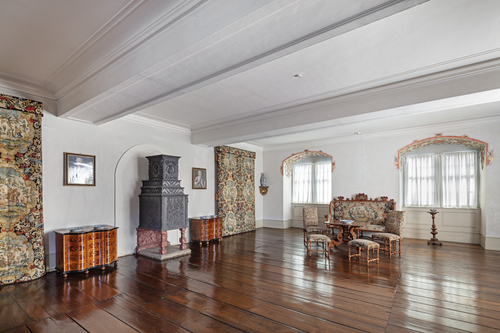
\includegraphics{tafelstube_files/figure-pdf/cell-4-output-2.png}

\begin{Shaded}
\begin{Highlighting}[]
\NormalTok{get\_text(}\StringTok{"Q264"}\NormalTok{)}
\CommentTok{\#Programm und Synthese der einstigen Tafelstube}
\end{Highlighting}
\end{Shaded}

Wikibase link:
\url{https://computational-publishing-service.wikibase.cloud/entity/Q264}

Kurator: Seeger, Ulrike

Programm und Synthese der einstigen Tafelstube

Tafelstube und Saal hängen konzeptionell eng zusammen. Während der Saal
mit der guten Herrschaft des Grafen Wolfgang einen regionalen Radius
beschreibt, weitet sich in der Tafelstube der Horizont auf den Beitrag
der Grafschaft Hohenlohe zur Rettung der Christenheit vor osmanischer
Herrschaft. Räumlich verknüpft sind die beiden Bildprogramme durch das
Relief des Innenportals mit der Belagerung von Gran (Eszergom) 1594 und
die Deckenmalerei des Durchgangs, die mit der Beweinung des toten Adonis
durch Venus und Amor auf den tragischen Tod des jüngsten Sohnes bei der
Belagerung von Gran (Eszergom) 1604 vorausweist. Adonis als
passionierter Jäger wiederum verband die Tafelstube mit dem Jagdzyklus
an der Decke des Saals.

\begin{Shaded}
\begin{Highlighting}[]
\NormalTok{get\_graph()}
\end{Highlighting}
\end{Shaded}

\begin{verbatim}
AttributeError: module 'numpy' has no attribute 'bool8'
---------------------------------------------------------------------------
AttributeError                            Traceback (most recent call last)
Cell In[5], line 1
----> 1 get_graph()

File /workspaces/tafelstube-notebook/funktionen.py:169, in get_graph()
    168 def get_graph():
--> 169     import VizKG.visualize as vkg
    170     results_graph1 = run_query(endpoint_url, query_graph)
    171     #print(results_graph1)
    172     #print('---')

File ~/.local/lib/python3.10/site-packages/VizKG/__init__.py:1
----> 1 from .visualize import *

File ~/.local/lib/python3.10/site-packages/VizKG/visualize.py:3
      1 import sys
      2 import random
----> 3 from .utils import set_chart, set_dataframe, chartdict
      4 from .charts import Chart
      5 class VizKG:

File ~/.local/lib/python3.10/site-packages/VizKG/utils/__init__.py:1
----> 1 from .util import *
      2 from .chartdict import chartdict

File ~/.local/lib/python3.10/site-packages/VizKG/utils/util.py:9
      6 from difflib import SequenceMatcher
      7 import ssl
----> 9 from .chartdict import chartdict as chart_dictionary
     11 def set_chart(chart_input):
     12     """
     13     Setter of chart based on chart input
     14 
   (...)
     17     :return: (str) chart: The available chart   
     18     """

File ~/.local/lib/python3.10/site-packages/VizKG/utils/chartdict.py:1
----> 1 from VizKG.charts import *
      2 """
      3 Dictionary of visualization charts 
      4 """
      5 chartdict = {
      6     'imagegrid': ImageGrid,
      7     'timeline': Timeline,
   (...)
     29     'radarchart': RadarChart
     30 }

File ~/.local/lib/python3.10/site-packages/VizKG/charts/__init__.py:7
      5 from .graph import Graph
      6 from .map import Map
----> 7 from .table import Table
      8 from .imagegrid import ImageGrid
      9 from .dimensions import Dimensions

File ~/.local/lib/python3.10/site-packages/VizKG/charts/table.py:2
      1 from .chart import Chart
----> 2 import plotly.figure_factory as ff
      3 from IPython.display import display
      4 import pandas as pd

File ~/.local/lib/python3.10/site-packages/plotly/figure_factory/__init__.py:32
     30 if optional_imports.get_module("pandas") is not None:
     31     from plotly.figure_factory._county_choropleth import create_choropleth
---> 32     from plotly.figure_factory._hexbin_mapbox import create_hexbin_mapbox
     33 else:
     35     def create_choropleth(*args, **kwargs):

File ~/.local/lib/python3.10/site-packages/plotly/figure_factory/_hexbin_mapbox.py:1
----> 1 from plotly.express._core import build_dataframe
      2 from plotly.express._doc import make_docstring
      3 from plotly.express._chart_types import choropleth_mapbox, scatter_mapbox

File ~/.local/lib/python3.10/site-packages/plotly/express/__init__.py:15
      9 if pd is None:
     10     raise ImportError(
     11         """\
     12 Plotly express requires pandas to be installed."""
     13     )
---> 15 from ._imshow import imshow
     16 from ._chart_types import (  # noqa: F401
     17     scatter,
     18     scatter_3d,
   (...)
     49     density_mapbox,
     50 )
     53 from ._core import (  # noqa: F401
     54     set_mapbox_access_token,
     55     defaults,
     56     get_trendline_results,
     57     NO_COLOR,
     58 )

File ~/.local/lib/python3.10/site-packages/plotly/express/_imshow.py:4
      2 from _plotly_utils.basevalidators import ColorscaleValidator
      3 from ._core import apply_default_cascade, init_figure, configure_animation_controls
----> 4 from .imshow_utils import rescale_intensity, _integer_ranges, _integer_types
      5 import pandas as pd
      6 import numpy as np

File ~/.local/lib/python3.10/site-packages/plotly/express/imshow_utils.py:24
      9 _integer_types = (
     10     np.byte,
     11     np.ubyte,  # 8 bits
   (...)
     19     np.ulonglong,
     20 )  # 64 bits
     21 _integer_ranges = {t: (np.iinfo(t).min, np.iinfo(t).max) for t in _integer_types}
     22 dtype_range = {
     23     np.bool_: (False, True),
---> 24     np.bool8: (False, True),
     25     np.float16: (-1, 1),
     26     np.float32: (-1, 1),
     27     np.float64: (-1, 1),
     28 }
     29 dtype_range.update(_integer_ranges)
     32 DTYPE_RANGE = dtype_range.copy()

File ~/.local/lib/python3.10/site-packages/numpy/__init__.py:410, in __getattr__(attr)
    407     import numpy.char as char
    408     return char.chararray
--> 410 raise AttributeError("module {!r} has no attribute "
    411                      "{!r}".format(__name__, attr))

AttributeError: module 'numpy' has no attribute 'bool8'
\end{verbatim}

\part{Belagerungsszenen des Langen Türkenkriegs an der Decke}

\begin{Shaded}
\begin{Highlighting}[]
\ImportTok{from}\NormalTok{ funktionen }\ImportTok{import} \OperatorTok{*}
\end{Highlighting}
\end{Shaded}

\begin{Shaded}
\begin{Highlighting}[]
\NormalTok{get\_text(}\StringTok{"Q278"}\NormalTok{)}
\CommentTok{\#Belagerungsszenen des Langen Türkenkrieges}
\end{Highlighting}
\end{Shaded}

Wikibase link:
\url{https://computational-publishing-service.wikibase.cloud/entity/Q278}

Kurator: Seeger, Ulrike

Belagerungsszenen des Langen Türkenkriegs an der Decke

Zuweisung der Gemälde in die einstige Tafelstube

Die einstige Deckenzier der Tafelstube ist den Inventaren, die ja
lediglich die mobilen Einrichtungsgegenstände aufführen, nicht zu
entnehmen. Einer Haustradition von Schloss Weikersheim zufolge waren an
der Decke ursprünglich jene 12 großformatigen Belagerungsszenen
angebracht, die sich heute in musealer Aufstellung teilweise im Flur vor
dem einstigen Appartement Graf Wolfgangs im Küchenbau befinden.{[}1{]}
Bei der Unterteilung des Raumes 1837 wurden sie abgenommen und tauchten
im Schloss 1946 wieder auf.{[}2{]} Ihre Anzahl, ihre Aufteilung in vier
schmale und acht breite Bilder sowie wie die exakten Maße{[}3{]} passen
sehr gut zu den Gefachen der Balkendecke. Es besteht also kein Anlass,
an dieser Haustradition zu zweifeln.

Urheberschaft und Datierung der Gemälde

Nahezu alle Gemälde sind stilistisch Balthasar Katzenberger
zuzuschreiben. Ein Vertrag wie der zu den Deckengemälden des Rittersaals
hat sich nicht erhalten, sodass sie nicht genau datiert sind. Sie
entstanden jedoch vermutlich sofort im Anschluss an die im November 1602
quittierten Deckengemälde des Saals, also von 1603 bis 1604. Bei der
spätesten dargestellten Belagerung von 1604 handelt es sich um einen
Nachzügler. Ihr Duktus ist nicht der von Katzenberger, was sich
insbesondere an den Wolkenformationen zeigt, die entgegen Katzenbergers
Gepflogenheit weiß konturiert sind. Möglicherweise ersetzte das Gemälde
ein anderes Bild und wurde zu einem Zeitpunkt gewünscht, als
Katzenberger nicht zur Verfügung stand. Der Anlass für die nachträgliche
Bestellung war der Tod von Graf Ludwig Kasimir bei der dargestellten
Belagerung von Gran im Jahr 1604, an die das Gemälde erinnert.

Komposition und Darstellungsmodus der Gemälde

Die hochrechteckigen Belagerungsszenen folgen im Aufbau prinzipiell den
achteckigen Jagdgemälden im Saal. Im Vordergrund hat Katzenberger ein
Getümmel inszeniert, das sich am unteren Bildrand abspielt und dessen
Protagonisten von beiden Seiten ins Bild reiten oder treten. Seitlich
wird das Geschehen von hohen Repoussoir-Bäume gerahmt, die sich am
oberen Bildrand durch die Beschriftung der Gemälde mit dunklen
Buchstaben vor blauem Himmel zu einer ovalen Rahmung zusammenschließen.
Im Mittel- und Hintergrund schilderte Katzenberger in weitläufiger
Landschaft die Belagerung einer Festung. Rings um die Festung stehen die
Zelte der Belagerer, entzünden sich Scharmützel und hin und wieder auch
kleinere Schlachten.

Thema, Vorlagen, Auswahl und Konzeption des Zyklus

Die Gemälde zeigen Belagerungen ungarischer Festungen, die sich während
des Langen Türkenkriegs ergaben. Der Lange Türkenkrieg begann 1593
zwischen dem Osmanischen Reich und den Habsburgern nachdem es schon
vorher auf beiden Seiten zu Grenzverletzungen gekommen war.{[}4{]} Es
handelte sich um einen Festungskrieg, bei dem die im Anschluss an die
osmanische Belagerung Wiens im Jahr 1529 auf beiden Seiten ausgebauten
Festungen wechselseitig belagert wurden. Beendet wurde der Krieg erst
1606 mit dem Frieden von Zsitvatorok. Die in Weikersheim dargestellten
Belagerungen beginnen angeblich schon 1590, spätestens jedoch 1594 und
reichen bis in das Jahr 1604.

Der Lange Türkenkrieg mit seinen vielen Belagerungen bestimmte bereits
das das Programm des inneren Ostportals des Rittersaals. Dieses Portal
führte nach Ansicht der Autorin nicht von der Tafelstube in den Saal,
sondern vom Saal in die Tafelstube. Es bereitete den Besucher des Saals
thematisch auf das Bildprogramm der Tafelstube vor, zumal das Portal und
die Deckengemälde der Tafelstube zur gleichen Zeit entstanden. Der
Stuckateur Gerhard Schmidt schuf sein 1603 signiertes und datiertes
Portal im Saal, während Katzenberger seine Gemälde in der Werkstatt
malte.

Als Vorlagen für die Belagerungsszenen im Hintergrund dienten
Kupferstiche, die einer ausführlichen, 1602 in Nürnberg erschienenen
Chronik über den Türkenkrieg beigebunden waren.{[}5{]} Verfasser des
Werkes „Chronologia oder Historische Beschreibung aller Kriegsemporungen
und Belägerungen der Stätt und Vestungen, auch Scharmützeln und
Schlachten, so in Ober- und Under-Ungarn, auch Sibenbürgen, mit dem
Türcken von A. 1395 biß auff gegenwertige Zeit gedenckhwürdig geschehen
\ldots``{[}6{]} war Hieronymus Oertl (Ortelius), der in Wien als
kaiserlicher Notar wegen seiner protestantischen Gesinnung 1580 in
Ungnade gefallen war und sich danach in Nürnberg niederließ.{[}7{]} Die
Anregung zu dem Werk ging von seinem Schwager, dem Nürnberger
Kupferstecher und Verleger Johann Sibmacher aus. Sibmacher zeichnete die
Belagerungsszenen nach Ortelius Vorgaben und stach sie in Kupfer.{[}8{]}

Die insgesamt 28 Kupfer wurden in der deutschsprachigen Legende in ihrem
Sujet genau benannt und mit dem Jahr der Belagerung versehen.
Katzenberger übernahm diese Beischriften buchstabengetreu für seine
Deckengemälde. Aufgrund der sehr genauen Übernahmen in Wort und Bild
kann man davon ausgehen, dass Ortelius` Chronik Graf Wolfgang im Jahr
ihres Erscheinens 1602 vorlag. Ausgewählt aus den 28 Kupfern wurden
Belagerungsaktionen sowohl der Kaiserlichen als auch der Osmanen. Harald
Drös, der sich bislang am ausführlichsten mit den Weikersheimer
Belagerungsszenen auseinandergesetzt hat und dem wertvolle Hinweise zu
verdanken sind,{[}9{]} vermutete deshalb sicher zurecht, dass die
Auswahl der Szenen davon bestimmt war, dass Mitglieder des Hauses
Hohenlohe beteiligt waren. Die folgende Beschreibung der Bilder
bestätigt diese Vermutung. Die späteste dargestellte Belagerung von Gran
(Eszergom), bei der der Sohn Ludwig Kasimir zu Tode kam,{[}10{]} bezieht
sich als ein Art Memorialbild auf dessen Tod. Auch dieses tragische
Ereignis wurde dem Besucher schon angekündigt, indem im Durchgang
zwischen Saal und Tafelstube die Beweinung des toten Adonis durch Venus
und Amor dargestellt wurde.

Drei der in Weikersheim dargestellten Belagerungen lagen später als das
Erscheinungsjahr der Chronik. Sie wurden hinzuerfunden und weisen
deutliche Schwächen in der Schilderung des Hintergrunds auf. Die drei
jeweils an der Donau stattgefundenen Aktionen wurden aus Landkarten und
Belagerungen Sibmachers versatzstückhaft kompiliert. Da die Gemälde
keinerlei Anhaltspunkte zu ihrer ursprünglichen Anordnung preisgeben,
folgt ihre nachfolgende Nummerierung der Chronologie der dargestellten
Belagerungen. Sie findet sich in der gleichen Reihenfolge zusammen mit
den genauen Maßen bei Harald Drös im Band der Inschriften des ehemaligen
Landkreises Mergentheim.{[}11{]}

Rekonstruktion der einstigen Anordnung

Bei der Rekonstruktion der Decke, die Jan Lutteroth miterarbeitet und
graphisch umgesetzt hat, wurde die Reihenfolge der durch keinerlei Bild-
oder Schriftquellen überlieferten Anbringung ebenfalls gemäß der
Chronologie gewählt. Die Geschichte beginnt in angenommener Leserichtung
von links nach rechts für den Eintretenden links oben mit dem
geheimnisvollen Nachtbild der Belagerung von Totis im Jahr 1590
(Belagerung I). Bei der Rekonstruktion der in vier Register
übereinanderliegenden Szenen musste lediglich im dritten Register einmal
die Chronologie verlassen werden, da die Belagerung der Stadt Waitzen im
Jahr 1597 (Belagerung VII) als schmales Bildformat nicht links außen,
sondern erst in der Mitte platziert werden konnte. Sie wird nun von den
Belagerungen von Raab 1598, wiederum einem effektvollen Nachtbild
(Belagerung VIII), und der Belagerung von Ofen ebenfalls im Jahr 1598
(Belagerung IX) flankiert.

Die drei Belagerungen, an denen Söhne teilgenommen hatten (Belagerung X,
XI, XII) stehen bei der gewählten Anordnung am Ende der Tafelstube. Die
drei darunterliegenden Fenster eröffnen den Blick auf die Stadt südlich
des Marktplatzes. Das besonders wichtige Gemälde mit dem bei der
Belagerung von Gran (Eszergom) 1604 getöteten Ludwig Kasimir (Belagerung
XII) kommt als letztes der Reihe rechts oben so zu stehen, dass Ludwig
Kasimir mit seinem Pferd Richtung Kirche reitet, wo er beigesetzt wurde.
Der trauernden Gräfin würde auf dem Gemälde ebenfalls der Weg zur Kirche
gewiesen.

{[}1{]} Merten, Weikersheim, o. J., S. 40. Trentin-Meyer, Georg
Friedrich von Hohenlohe, 2019, S. 90 spricht versehentlich von 13
Gemälden.

{[}2{]} Freeden, Kamin, 1950, S. 142.

{[}3{]} Die Maße bei Drös, Inschriften Mergentheim, 2002, S. 248. Ebd.,
S. 249 die bislang ausführlichste Auseinandersetzung mit den Gemälden.

{[}4{]} Zum Langen Türkenkrieg: Niederkorn, Langer Türkenkrieg, 1993.

{[}5{]} Diese wichtige Vorlage bereits bei Fandrey, Weikersheim, 2010,
S. 60.

{[}6{]} Ortelius, Chronologia, 1602.

{[}7{]} Mummenhoff, Ernst, ``Oertl, Hieronymus'' in: Allgemeine Deutsche
Biographie 24 (1887), S. 445-446 {[}Online-Version{]}; URL:
https://www.deutsche-biographie.de/pnd128534958.html\#adbcontent.

{[}8{]} Ebd. Außerdem Ortelius, Chronologia, 1602, „Ad Lectorem``.

{[}9{]} Drös, Inschriften Mergentheim, 2002, S. 248--249.

{[}10{]} Drös, Inschriften Mergentheim, 2002, S. 248--250.

{[}11{]} Drös, Inschriften Mergentheim, 2002, Nr. 366.

\chapter{Belagerungsszene I: Eroberung der Festung
Tottis}\label{belagerungsszene-i-eroberung-der-festung-tottis}

\begin{Shaded}
\begin{Highlighting}[]
\ImportTok{from}\NormalTok{ funktionen }\ImportTok{import} \OperatorTok{*}
\end{Highlighting}
\end{Shaded}

\begin{Shaded}
\begin{Highlighting}[]
\NormalTok{get\_text(}\StringTok{"Q252"}\NormalTok{)}
\CommentTok{\#Belagerungsszene I}

\NormalTok{get\_img(}\StringTok{"Q238"}\NormalTok{)}
\CommentTok{\#Vestung Tottis}
\end{Highlighting}
\end{Shaded}

Wikibase link:
\url{https://computational-publishing-service.wikibase.cloud/entity/Q252}

Kurator: Seeger, Ulrike

Belagerung I: „Vestung Tottis, wie die von den Christen bei der Nacht
erobert worden, 1590``

Breites Format. Vorne rechts ins Bild hineinreitende Reiter mit großen
Fahnen. Im Hintergrund die ungarische Festung Totis (Tata) nach dem
Vorbild von Sibmachers Kupferstich, der allerdings eine Eroberung durch
die Christen aus dem Jahr 1597 wiedergibt. Die sehr dunkle Szenerie wird
von zwei Laternen spärlich erleuchtet. Da Totis nicht 1590, sondern 1597
und 1598 durch die Christen erobert wurde, und zudem zu den zeitlich als
nächste dargestellten Belagerungen eine Zeitspanne von vier Jahren
liegt, kann es gut sein, dass der Jahreszahl 1590 ein Versehen zugrunde
liegt.

Wikibase link:
\url{https://computational-publishing-service.wikibase.cloud/entity/Q265}

Title: Eroberung der Festung Tottis -- Gesamtansicht

Year: 2018

Description: Teil von: Wanddekoration des Flurs \& Raum 73a
Belagerungsszenen und Türkenschlachten; Balthasar Kazenberger, Maler -
Weikersheim, Schloss Weikersheim, Flur \& Raum 73a - 1603-1604

\includegraphics{belagerung_01_files/figure-pdf/cell-3-output-2.png}

\chapter{Belagerungsszene II: Belagerung der Festung
Gran}\label{belagerungsszene-ii-belagerung-der-festung-gran}

\begin{Shaded}
\begin{Highlighting}[]
\ImportTok{from}\NormalTok{ funktionen }\ImportTok{import} \OperatorTok{*}
\end{Highlighting}
\end{Shaded}

\begin{Shaded}
\begin{Highlighting}[]
\NormalTok{get\_text(}\StringTok{"Q253"}\NormalTok{)}
\CommentTok{\#Belagerung II}

\NormalTok{get\_img(}\StringTok{"Q239"}\NormalTok{)}
\CommentTok{\#Festung Gran}
\end{Highlighting}
\end{Shaded}

Wikibase link:
\url{https://computational-publishing-service.wikibase.cloud/entity/Q253}

Kurator: Seeger, Ulrike

Belagerung II: „Vestung Gran wie die von Christen belegert gewesen.
1594``

Schmales Format. Vorne links ein Hellebardier mit einem Knecht, der mit
schwarzen Kugeln als Munition hantiert. Von rechts kommt dynamisch ein
Reiter mit rotem Mantel, schwarzem Zylinder und möglicherweise einer
Trompete im Arm ins Bild geritten. Da an der versuchten Einnahme von
Gran (Eszergom) im Jahr 1594 Graf Georg Friedrich, der älteste Sohn von
Graf Wolfgang II., als kaiserlicher Obrist beteiligt war,{[}1{]} darf
man den Reiter im roten Mantel vermutlich mit diesem identifizieren.
Sein Gesicht folgt mit hellem Teint, roten Bäckchen, hoher Stirn,
Schnauzbart und fein geschwungenen Augenbrauen dem des Grafen Wolfgang
auf den Deckengemälden des Rittersaals mit dem Unterschied, dass es von
dunkelbraunem Haar gerahmt wird.

Im Mittelgrund blickt man auf das Feldlager der kaiserlichen Armee. Von
einer Verschanzung in den Donauauen wird am gegenüberliegenden Ufer die
Wasserstadt von Gran beschossen. Darüber liegt die Festung Gran mit der
Doppelturmfassade der Kathedrale. Mehrere Minarette deuten die türkische
Herrschaft an. Die Ansicht folgt nicht dem Kupferstich von Sibmacher,
der Gran von einem anderen Blickwinkel und zudem summarischer zeigt.
Ohnehin hat Sibmacher nicht die Belagerung des Jahres 1594, sondern die
des Jahres 1595 dargestellt. Da Georg Friedrich an dem Ereignis 1594
beteiligt war, dürfte die Weikersheimer Darstellung auf Flugblätter oder
bebilderte Zeitungsberichte zurückgehen, die es mannigfach zu den
Ereignissen des Langen Türkenkriegs gab. Der von links mit einer Drehung
ins Bild hineinreitende Reiter hat sein Vorbild in einem Stich von
Stradanus zur Wolfsjagd (Nachdruck Olms, Tf. 20).

{[}1{]} Trentin-Meyer, Georg Friedrich von Hohenlohe, 2019, S. 90.

Wikibase link:
\url{https://computational-publishing-service.wikibase.cloud/entity/Q266}

Title: Belagerung der Festung Gran -- Gesamtansicht (1594)

Year: 2018

Description: Teil von: Wanddekoration des Flurs \& Raum 73a
Belagerungsszenen und Türkenschlachten; Balthasar Kazenberger, Maler -
Weikersheim, Schloss Weikersheim, Flur \& Raum 73a - 1603-1604

\includegraphics{belagerung_02_files/figure-pdf/cell-3-output-2.png}

\chapter{Belagerungsszene III: Belagerung der Festung
Raab}\label{belagerungsszene-iii-belagerung-der-festung-raab}

\begin{Shaded}
\begin{Highlighting}[]
\ImportTok{from}\NormalTok{ funktionen }\ImportTok{import} \OperatorTok{*}
\end{Highlighting}
\end{Shaded}

\begin{Shaded}
\begin{Highlighting}[]
\NormalTok{get\_text(}\StringTok{"Q254"}\NormalTok{)}
\CommentTok{\#Belagerung III}

\NormalTok{get\_img(}\StringTok{"Q240"}\NormalTok{)}
\CommentTok{\#Festung Raab}
\end{Highlighting}
\end{Shaded}

Wikibase link:
\url{https://computational-publishing-service.wikibase.cloud/entity/Q254}

Kurator: Seeger, Ulrike

Belagerung III: „Vestung Raab, wie die vom Türcken belegert gewesen.
A{[}nn{]}o 1594''

Breites Format. Von rechts kommen türkische Reiter ins Bild. Im
Mittelgrund ist am gegenüberliegenden Ufer der Donau die quadratische
Festung Raab (Győr) zu erkennen. Ihre Eckbastionen und die Bastion an
einer links zusätzlich stumpfwinkelig vorstoßenden Ecke sind mit Kanonen
besetzt. Die vom Feldlager der Türken umzingelte Festung wird heftig
beschossen. Im Vordergrund spielt sich am linken unteren Bildrand ein
Nahkampf zwischen Christen und Türken ab, der sich neben zwei
Transportkutschen entzündet hat. Die Darstellung der Festung und der
Kampfhandlungen folgt getreu der Vorlage bei Ortelius.

Wikibase link:
\url{https://computational-publishing-service.wikibase.cloud/entity/Q267}

Title: Belagerung der Festung Raab -- Gesamtansicht

Year: 2018

Description: Teil von: Wanddekoration des Flurs \& Raum 73a
Belagerungsszenen und Türkenschlachten; Balthasar Kazenberger, Maler -
Weikersheim, Schloss Weikersheim, Flur \& Raum 73a - 1603-1604

\includegraphics{belagerung_03_files/figure-pdf/cell-3-output-2.png}

\chapter{Belagerungsszene IV: Belagerung der Festung
Comorna}\label{belagerungsszene-iv-belagerung-der-festung-comorna}

\begin{Shaded}
\begin{Highlighting}[]
\ImportTok{from}\NormalTok{ funktionen }\ImportTok{import} \OperatorTok{*}
\end{Highlighting}
\end{Shaded}

\begin{Shaded}
\begin{Highlighting}[]
\NormalTok{get\_text(}\StringTok{"Q255"}\NormalTok{)}
\CommentTok{\#Belagerung IV}

\NormalTok{get\_img(}\StringTok{"Q241"}\NormalTok{)}
\CommentTok{\#Festung Comorna}
\end{Highlighting}
\end{Shaded}

Wikibase link:
\url{https://computational-publishing-service.wikibase.cloud/entity/Q255}

Kurator: Seeger, Ulrike

Belagerung IV: „Vestung Comorna wie die vom Türckn belegert
gewe{[}sen{]} 1594``

Breites Format. Von links kommen türkische Reiter ins Bild, von denen
ein blau gekleideter Frontmann eine lange Lanze mit blauer Fahne
dynamisch diagonal ins Bild stößt. Rechts unten knien vor türkischen
Zelten zwei Dromedare. Den Höcker des vorderen Dromedars bedeckt ein
blaues Tuch mit aufgesticktem Sonnensymbol. Der Mittelgrund ist durch
den Verlauf der Donau zweigeteilt. Am Ufer im Vordergrund formiert sich
ein türkisches Heer. Auf der gegenüberliegenden Seite liegt die von den
Christen gehaltene Festung von Komorn (Komárom). Sie überstand die
Belagerung unversehrt, während die hinter der Festung anschließende
Stadt in Flammen steht.

Die Festung Komorn besetzte eine Landspitze an der Mündung der Waag in
die Donau. Sie wurde von dem kaiserlichen Festungsbaumeister Pietro
Ferrabosco unterstützt durch Daniel Specklin auf einem dreieckigen
Grundriss angelegt. Die türkische Belagerung 1594 überstand sie
unversehrt. In der Folgezeit wurde sie verstärkt und weiterhin nicht
eingenommen. Mit der Darstellung der Festung und der brennenden Stadt
Komorn folgte Katzenberger treu dem Vorbild Sibmachers. Die Anregung zu
den beiden Dromedaren im Vordergrund erhielt er ebenfalls von Sibmacher,
der die Dromedare als Reittiere der Osmanen im Vordergrund allerdings
nur klein darstellte.

Wikibase link:
\url{https://computational-publishing-service.wikibase.cloud/entity/Q268}

Title: Belagerung der Festung Comorna -- Gesamtansicht

Year: 2018

Description: Teil von: Wanddekoration des Flurs \& Raum 73a
Belagerungsszenen und Türkenschlachten; Balthasar Kazenberger, Maler -
Weikersheim, Schloss Weikersheim, Flur \& Raum 73a - 1603-1604

\includegraphics{belagerung_04_files/figure-pdf/cell-3-output-2.png}

\chapter{Belagerungsszene V: Eroberung der Festung
Gran}\label{belagerungsszene-v-eroberung-der-festung-gran}

\begin{Shaded}
\begin{Highlighting}[]
\ImportTok{from}\NormalTok{ funktionen }\ImportTok{import} \OperatorTok{*}
\end{Highlighting}
\end{Shaded}

\begin{Shaded}
\begin{Highlighting}[]
\NormalTok{get\_text(}\StringTok{"Q256"}\NormalTok{)}
\CommentTok{\#Belagerung V}

\NormalTok{get\_img(}\StringTok{"Q242"}\NormalTok{)}
\CommentTok{\#Festung Gran}
\end{Highlighting}
\end{Shaded}

Wikibase link:
\url{https://computational-publishing-service.wikibase.cloud/entity/Q256}

Kurator: Seeger, Ulrike

Belagerung V: „Vestung Gran wie die von den Christen wider erobert
worden. A{[}nn{]}o 1595.``

Breites Format. Im Vordergrund links beugt sich eine Rückenfigur nach
vorne, sodass sie dem Betrachter den Hintern zeigt. Am rechten unteren
Bildrand steht die Halbfigur eines Höflings mit Flinte und braunem
Pferd. Dem Gesicht nach zu urteilen, handelt es sich um einen der Söhne
von Graf Wolfgang. Im Mittelgrund ist eine Schlacht mit türkischen
Reitern mit langen Lanzen zu sehen. Den Hintergrund bildet eine im
Dunkeln liegende Hügellandschaft, in der auf einem Berg die Festung Gran
(Győr), am Ufer der Donau die zugehörige Wasserstadt und vor allem die
ebenfalls befestigte Ratzenstadt (Rácvázószöveg) gut zu erkennen sind.
Die Landschaft folgt treu der Vorlage bei Ortelius.

Die Fahnen lassen den Stand der Eroberung erkennen, was sich dem
heutigen Betrachter nur noch mithilfe der Erläuterungen auf dem
Kupferstich bei Ortelius erschließt. Über der Festung Gran, die laut
Ortelius am 3. August eingenommen wurde, weht klein noch die türkische
Fahne mit einer gelben Sonne auf rotem Grund. Über der Ratzenstadt, die
im Juli als erstes erobert wurde, weht groß die Fahne der Kaiserlichen
mit gewelltem weißem Andreaskreuz auf rotem Grund. Die Wasserstadt, über
der bei Katzenberger die kaiserliche Fahne mit dem Reichsadler auf
goldenem Grund steht, wurde laut Ortelius Ende August erobert, sodass
mit Ende August der zur Darstellung gelangte Zeitpunkt getroffen sein
dürfte.

Wikibase link:
\url{https://computational-publishing-service.wikibase.cloud/entity/Q269}

Title: Eroberung der Festung Gran -- Gesamtansicht

Year: 2018

Description: Teil von: Wanddekoration des Flurs \& Raum 73a
Belagerungsszenen und Türkenschlachten; Balthasar Kazenberger, Maler -
Weikersheim, Schloss Weikersheim, Flur \& Raum 73a - 1603-1604

\begin{verbatim}
ConnectTimeout: HTTPSConnectionPool(host='previous.bildindex.de', port=443): Max retries exceeded with url: /bilder/fmd10005848a.jpg (Caused by ConnectTimeoutError(<urllib3.connection.HTTPSConnection object at 0x73f0c43f0cd0>, 'Connection to previous.bildindex.de timed out. (connect timeout=None)'))
---------------------------------------------------------------------------
TimeoutError                              Traceback (most recent call last)
File ~/.local/lib/python3.10/site-packages/urllib3/connection.py:196, in HTTPConnection._new_conn(self)
    195 try:
--> 196     sock = connection.create_connection(
    197         (self._dns_host, self.port),
    198         self.timeout,
    199         source_address=self.source_address,
    200         socket_options=self.socket_options,
    201     )
    202 except socket.gaierror as e:

File ~/.local/lib/python3.10/site-packages/urllib3/util/connection.py:85, in create_connection(address, timeout, source_address, socket_options)
     84 try:
---> 85     raise err
     86 finally:
     87     # Break explicitly a reference cycle

File ~/.local/lib/python3.10/site-packages/urllib3/util/connection.py:73, in create_connection(address, timeout, source_address, socket_options)
     72     sock.bind(source_address)
---> 73 sock.connect(sa)
     74 # Break explicitly a reference cycle

TimeoutError: [Errno 110] Connection timed out

The above exception was the direct cause of the following exception:

ConnectTimeoutError                       Traceback (most recent call last)
File ~/.local/lib/python3.10/site-packages/urllib3/connectionpool.py:789, in HTTPConnectionPool.urlopen(self, method, url, body, headers, retries, redirect, assert_same_host, timeout, pool_timeout, release_conn, chunked, body_pos, preload_content, decode_content, **response_kw)
    788 # Make the request on the HTTPConnection object
--> 789 response = self._make_request(
    790     conn,
    791     method,
    792     url,
    793     timeout=timeout_obj,
    794     body=body,
    795     headers=headers,
    796     chunked=chunked,
    797     retries=retries,
    798     response_conn=response_conn,
    799     preload_content=preload_content,
    800     decode_content=decode_content,
    801     **response_kw,
    802 )
    804 # Everything went great!

File ~/.local/lib/python3.10/site-packages/urllib3/connectionpool.py:490, in HTTPConnectionPool._make_request(self, conn, method, url, body, headers, retries, timeout, chunked, response_conn, preload_content, decode_content, enforce_content_length)
    489         new_e = _wrap_proxy_error(new_e, conn.proxy.scheme)
--> 490     raise new_e
    492 # conn.request() calls http.client.*.request, not the method in
    493 # urllib3.request. It also calls makefile (recv) on the socket.

File ~/.local/lib/python3.10/site-packages/urllib3/connectionpool.py:466, in HTTPConnectionPool._make_request(self, conn, method, url, body, headers, retries, timeout, chunked, response_conn, preload_content, decode_content, enforce_content_length)
    465 try:
--> 466     self._validate_conn(conn)
    467 except (SocketTimeout, BaseSSLError) as e:

File ~/.local/lib/python3.10/site-packages/urllib3/connectionpool.py:1095, in HTTPSConnectionPool._validate_conn(self, conn)
   1094 if conn.is_closed:
-> 1095     conn.connect()
   1097 # TODO revise this, see https://github.com/urllib3/urllib3/issues/2791

File ~/.local/lib/python3.10/site-packages/urllib3/connection.py:615, in HTTPSConnection.connect(self)
    614 sock: socket.socket | ssl.SSLSocket
--> 615 self.sock = sock = self._new_conn()
    616 server_hostname: str = self.host

File ~/.local/lib/python3.10/site-packages/urllib3/connection.py:205, in HTTPConnection._new_conn(self)
    204 except SocketTimeout as e:
--> 205     raise ConnectTimeoutError(
    206         self,
    207         f"Connection to {self.host} timed out. (connect timeout={self.timeout})",
    208     ) from e
    210 except OSError as e:

ConnectTimeoutError: (<urllib3.connection.HTTPSConnection object at 0x73f0c43f0cd0>, 'Connection to previous.bildindex.de timed out. (connect timeout=None)')

The above exception was the direct cause of the following exception:

MaxRetryError                             Traceback (most recent call last)
File ~/.local/lib/python3.10/site-packages/requests/adapters.py:667, in HTTPAdapter.send(self, request, stream, timeout, verify, cert, proxies)
    666 try:
--> 667     resp = conn.urlopen(
    668         method=request.method,
    669         url=url,
    670         body=request.body,
    671         headers=request.headers,
    672         redirect=False,
    673         assert_same_host=False,
    674         preload_content=False,
    675         decode_content=False,
    676         retries=self.max_retries,
    677         timeout=timeout,
    678         chunked=chunked,
    679     )
    681 except (ProtocolError, OSError) as err:

File ~/.local/lib/python3.10/site-packages/urllib3/connectionpool.py:843, in HTTPConnectionPool.urlopen(self, method, url, body, headers, retries, redirect, assert_same_host, timeout, pool_timeout, release_conn, chunked, body_pos, preload_content, decode_content, **response_kw)
    841     new_e = ProtocolError("Connection aborted.", new_e)
--> 843 retries = retries.increment(
    844     method, url, error=new_e, _pool=self, _stacktrace=sys.exc_info()[2]
    845 )
    846 retries.sleep()

File ~/.local/lib/python3.10/site-packages/urllib3/util/retry.py:519, in Retry.increment(self, method, url, response, error, _pool, _stacktrace)
    518     reason = error or ResponseError(cause)
--> 519     raise MaxRetryError(_pool, url, reason) from reason  # type: ignore[arg-type]
    521 log.debug("Incremented Retry for (url='%s'): %r", url, new_retry)

MaxRetryError: HTTPSConnectionPool(host='previous.bildindex.de', port=443): Max retries exceeded with url: /bilder/fmd10005848a.jpg (Caused by ConnectTimeoutError(<urllib3.connection.HTTPSConnection object at 0x73f0c43f0cd0>, 'Connection to previous.bildindex.de timed out. (connect timeout=None)'))

During handling of the above exception, another exception occurred:

ConnectTimeout                            Traceback (most recent call last)
Cell In[2], line 4
      1 get_text("Q256")
      2 #Belagerung V
----> 4 get_img("Q242")
      5 #Festung Gran

File /workspaces/tafelstube-notebook/funktionen.py:163, in get_img(partOfItem_id)
    161 image_url=item['imgUrl']['value']
    162 headers = {'User-Agent': 'Ex_Books_conference_bot/0.0 (https://github.com/SimonXIX/Experimental_Books_workshop; ad7588@coventry.ac.uk)'}
--> 163 im = fetch_image_by_url(image_url, headers)
    164 im.thumbnail((500, 500), Image.Resampling.LANCZOS)
    165 display(im)

File /workspaces/tafelstube-notebook/funktionen.py:132, in fetch_image_by_url(url, headers)
    131 def fetch_image_by_url(url, headers):
--> 132     r = requests.get(url, headers=headers, stream=True)
    133     if r.status_code == 200:
    134         im = Image.open(r.raw)

File ~/.local/lib/python3.10/site-packages/requests/api.py:73, in get(url, params, **kwargs)
     62 def get(url, params=None, **kwargs):
     63     r"""Sends a GET request.
     64 
     65     :param url: URL for the new :class:`Request` object.
   (...)
     70     :rtype: requests.Response
     71     """
---> 73     return request("get", url, params=params, **kwargs)

File ~/.local/lib/python3.10/site-packages/requests/api.py:59, in request(method, url, **kwargs)
     55 # By using the 'with' statement we are sure the session is closed, thus we
     56 # avoid leaving sockets open which can trigger a ResourceWarning in some
     57 # cases, and look like a memory leak in others.
     58 with sessions.Session() as session:
---> 59     return session.request(method=method, url=url, **kwargs)

File ~/.local/lib/python3.10/site-packages/requests/sessions.py:589, in Session.request(self, method, url, params, data, headers, cookies, files, auth, timeout, allow_redirects, proxies, hooks, stream, verify, cert, json)
    584 send_kwargs = {
    585     "timeout": timeout,
    586     "allow_redirects": allow_redirects,
    587 }
    588 send_kwargs.update(settings)
--> 589 resp = self.send(prep, **send_kwargs)
    591 return resp

File ~/.local/lib/python3.10/site-packages/requests/sessions.py:703, in Session.send(self, request, **kwargs)
    700 start = preferred_clock()
    702 # Send the request
--> 703 r = adapter.send(request, **kwargs)
    705 # Total elapsed time of the request (approximately)
    706 elapsed = preferred_clock() - start

File ~/.local/lib/python3.10/site-packages/requests/adapters.py:688, in HTTPAdapter.send(self, request, stream, timeout, verify, cert, proxies)
    685 if isinstance(e.reason, ConnectTimeoutError):
    686     # TODO: Remove this in 3.0.0: see #2811
    687     if not isinstance(e.reason, NewConnectionError):
--> 688         raise ConnectTimeout(e, request=request)
    690 if isinstance(e.reason, ResponseError):
    691     raise RetryError(e, request=request)

ConnectTimeout: HTTPSConnectionPool(host='previous.bildindex.de', port=443): Max retries exceeded with url: /bilder/fmd10005848a.jpg (Caused by ConnectTimeoutError(<urllib3.connection.HTTPSConnection object at 0x73f0c43f0cd0>, 'Connection to previous.bildindex.de timed out. (connect timeout=None)'))
\end{verbatim}

\chapter{Belagerungsszene VI: Belagerung der Festung von
Visegrád}\label{belagerungsszene-vi-belagerung-der-festung-von-visegruxe1d}

\begin{Shaded}
\begin{Highlighting}[]
\ImportTok{from}\NormalTok{ funktionen }\ImportTok{import} \OperatorTok{*}
\end{Highlighting}
\end{Shaded}

\begin{Shaded}
\begin{Highlighting}[]
\NormalTok{get\_text(}\StringTok{"Q257"}\NormalTok{)}
\CommentTok{\#Belagerung VI}

\NormalTok{get\_img(}\StringTok{"Q243"}\NormalTok{)}
\CommentTok{\#Festung Visegrád}
\end{Highlighting}
\end{Shaded}

Wikibase link:
\url{https://computational-publishing-service.wikibase.cloud/entity/Q257}

Kurator: Seeger, Ulrike

Belagerung VI: ``Vestung Vizzegrad wie die von Christen belegert gewesen
Anno 1595``

Breites Format. Im Vordergrund stehen in der linken Bildhälfte zwei
prächtig gekleidete Offiziere, einer als Rückenfigur mit Rüstung und
Federbusch, einer mit grau schimmerndem Gewand und auffälligem Helm.
Derjenige im grauen Gewand wendet den Blick dem Betrachter zu. Da an der
Belagerung der Neffe von Papst Clemens VIII., Giovanni Francesco
Aldobrandini, beteiligt war, könnte es sich um diesen und einen
Begleiter handeln. Rechts vorne machen sich Männer an Kanonen zu
schaffen. Im Hintergrund erhebt sich charakteristisch auf einem
kegelförmigen Berg am Ufer der Donau die Zitadelle von Visegrád. Sie
beherrscht einen großen natürlichen Hafen mit zahlreichen
Transportschiffen. Das Gemälde lebt stimmungsvoll von silbrigen
Grautönen, aus denen vereinzelt rote Fahnen und andere Details rot
herausleuchten.

Wikibase link:
\url{https://computational-publishing-service.wikibase.cloud/entity/Q270}

Title: Belagerung der Festung von Visegrád -- Gesamtansicht

Year: 2018

Description: Teil von: Wanddekoration des Flurs \& Raum 73a
Belagerungsszenen und Türkenschlachten; Balthasar Kazenberger, Maler -
Weikersheim, Schloss Weikersheim, Flur \& Raum 73a - 1603-1604

\includegraphics{belagerung_06_files/figure-pdf/cell-3-output-2.png}

\chapter{Belagerungsszene VII: Belagerung der Stadt
Waitzen}\label{belagerungsszene-vii-belagerung-der-stadt-waitzen}

\begin{Shaded}
\begin{Highlighting}[]
\ImportTok{from}\NormalTok{ funktionen }\ImportTok{import} \OperatorTok{*}
\end{Highlighting}
\end{Shaded}

\begin{Shaded}
\begin{Highlighting}[]
\NormalTok{get\_text(}\StringTok{"Q258"}\NormalTok{)}
\CommentTok{\#Belagerung VII}

\NormalTok{get\_img(}\StringTok{"Q244"}\NormalTok{)}
\CommentTok{\#Stadt Waitzen}
\end{Highlighting}
\end{Shaded}

Wikibase link:
\url{https://computational-publishing-service.wikibase.cloud/entity/Q258}

Kurator: Seeger, Ulrike

Belagerung VII: „Statt Waitzen wie die von vom Türcken belegert gewesen
1597``

Schmales Format. Rechts im Vordergrund reitet ein Türke mit Turban und
Streitkolben frontal auf den Betrachter zu. Links unter ihm steht ein
türkisches Zelt. Im Hintergrund liegt an der Donau Waitzen (Vác), das
sich aus einer befestigten Stadt und einem befestigten Kloster
zusammensetzt. In der Stadt, an deren Rand sich eine Moschee befindet,
brennen mehrere Häuser. Verglichen mit dem Kupferstich bei Ortelius sind
Stadt und Kloster seitenverkehrt dargestellt.

Wikibase link:
\url{https://computational-publishing-service.wikibase.cloud/entity/Q271}

Title: Belagerung der Stadt Waitzen -- Gesamtansicht

Year: 2018

Description: Teil von: Wanddekoration des Flurs \& Raum 73a
Belagerungsszenen und Türkenschlachten; Balthasar Kazenberger, Maler -
Weikersheim, Schloss Weikersheim, Flur \& Raum 73a - 1603-1604

\includegraphics{belagerung_07_files/figure-pdf/cell-3-output-2.png}

\chapter{Belagerungsszene VIII: Wiedereroberung der Festung
Raab}\label{belagerungsszene-viii-wiedereroberung-der-festung-raab}

\begin{Shaded}
\begin{Highlighting}[]
\ImportTok{from}\NormalTok{ funktionen }\ImportTok{import} \OperatorTok{*}
\end{Highlighting}
\end{Shaded}

\begin{Shaded}
\begin{Highlighting}[]
\NormalTok{get\_text(}\StringTok{"Q259"}\NormalTok{)}
\CommentTok{\#Belagerung VIII}

\NormalTok{get\_img(}\StringTok{"Q245"}\NormalTok{)}
\CommentTok{\#Wiedereroberung Raab }
\end{Highlighting}
\end{Shaded}

\begin{verbatim}
NameError: name 'get_text' is not defined
---------------------------------------------------------------------------
NameError                                 Traceback (most recent call last)
Cell In[1], line 1
----> 1 get_text("Q259")
      2 #Belagerung VIII
      4 get_img("Q245")

NameError: name 'get_text' is not defined
\end{verbatim}

\chapter{Belagerungsszene IX: Belagerung der Stadt Ofen im Jahr
1598}\label{belagerungsszene-ix-belagerung-der-stadt-ofen-im-jahr-1598}

\begin{Shaded}
\begin{Highlighting}[]
\ImportTok{from}\NormalTok{ funktionen }\ImportTok{import} \OperatorTok{*}
\end{Highlighting}
\end{Shaded}

\begin{Shaded}
\begin{Highlighting}[]
\NormalTok{get\_text(}\StringTok{"Q260"}\NormalTok{)}
\CommentTok{\#Belagerung IX}

\NormalTok{get\_img(}\StringTok{"Q246"}\NormalTok{)}
\CommentTok{\#Stadt Ofen 1598}
\end{Highlighting}
\end{Shaded}

Wikibase link:
\url{https://computational-publishing-service.wikibase.cloud/entity/Q260}

Kurator: Seeger, Ulrike

Belagerung IX: „Hauptstatt Offen. wie die von Christen belegert gewesen.
1598.``

Breites Format. Im Vordergrund steht eine große Kanone, die von Pferden
nach links aus dem Bild gezogen wird. Auf der Kanone sitzt der Kutscher
mit Pelzmütze, mongolisch anmutendem Bart und rotem Mantel. Er schwingt
eine lange Peitsche. Am rechten Bildrand steht ein junger, ebenfalls
mongolisch aussehender Mann in einem hellen Wams. Hinter der fahrenden
Kanone rennt ein Jagdhund her.

Im Hintergrund erstreckt sich Ofen (Óbuda, heute Buda als Stadtteil von
Budapest) als prächtige Stadt mit hoher Stadtmauer, einem Schloss,
zahlreichen Kirchen und Minaretten sowie außerhalb der Mauern einem
Lustgarten mit Pavillon. Der Lustgarten ist dem Schloss, auf dem bei
Ortelius eine türkische Fahne weht, unmittelbar vorgelagert. Im
Mittelgrund liegt ebenfalls außerhalb der Stadtmauern ein türkischer
Friedhof mit zahlreichen Grabsteinen und einem runden gedrungenen Turm
in der Mitte. Katzenberger hat die Stadtansicht mitsamt der Schilderung
des Lustgartens und des Friedhofs von Sibmacher übernommen.

Wikibase link:
\url{https://computational-publishing-service.wikibase.cloud/entity/Q273}

Title: Belagerung der Stadt Ofen im Jahr 1598 -- Gesamtansicht

Year: 2018

Description: Teil von: Wanddekoration des Flurs \& Raum 73a
Belagerungsszenen und Türkenschlachten; Balthasar Kazenberger, Maler -
Weikersheim, Schloss Weikersheim, Flur \& Raum 73a - 1603-1604

\includegraphics{belagerung_09_files/figure-pdf/cell-3-output-2.png}

\chapter{Belagerungsszene X: Belagerung der Stadt Ofen im Jahr
1603}\label{belagerungsszene-x-belagerung-der-stadt-ofen-im-jahr-1603}

\begin{Shaded}
\begin{Highlighting}[]
\ImportTok{from}\NormalTok{ funktionen }\ImportTok{import} \OperatorTok{*}
\end{Highlighting}
\end{Shaded}

\begin{Shaded}
\begin{Highlighting}[]
\NormalTok{get\_text(}\StringTok{"Q261"}\NormalTok{)}
\CommentTok{\#Belagerung X}

\NormalTok{get\_img(}\StringTok{"Q247"}\NormalTok{)}
\CommentTok{\#Stadt Ofen 1603}
\end{Highlighting}
\end{Shaded}

Wikibase link:
\url{https://computational-publishing-service.wikibase.cloud/entity/Q261}

Kurator: Seeger, Ulrike

Belagerung X: „Hauptstatt Offen, wie die von Christen belegert gewesen.
Anno 1603``

Breites Format. Vorne rechts reitet auf einem grauen Pferd ein
gerüsteter kaiserlicher Heerführer mit weißem Federbusch ins Bild.
Seinem Gesichtsschnitt und dem blonden Bart zufolge handelt es sich um
einen Sohn von Graf Wolfgang. Vor ihm läuft ein Knappe mit prächtigem
roten Mantel, rotem Federbusch und einem Gewehr über der Schulter. Er
weist ihm den Weg zum Feldlager. Hinter dem Feldlager stehen auf der
anderen Seite eines Donauzuflusses Truppen in Aufstellung. An einer
Verschanzung werden Kanonen gezündet. Der Geländezipfel zwischen Donau
und Zufluss ist mit einer dreieckigen Festung besetzt, zu der sich eine
Schiffbrücke spannt. Die in der vorangegangenen Belagerung von Ofen aus
dem Jahr 1598 prächtig geschilderte Stadt Ofen (Óbuda, heute Buda als
Stadtteil von Budapest) befindet sich auf dem Gemälde angeschnitten am
linken Bildrand. Sie ist an den vorgelagerten Donauinseln zu erkennen,
auf die weitere Schiffbrücken führen.

Katzenberger konnte für die Belagerung von 1703 nicht mehr auf Ortelius
zurückgreifen, dessen Werk 1702 erschien. Vermutlich orientierte er sich
an Schilderungen des Sohnes und übernahm die Flussmündung mit der
dreieckigen Festung aus der Darstellung einer anderen Belagerung, da sie
sich auf Karten der Donau bei Buda nicht finden lässt.

Wikibase link:
\url{https://computational-publishing-service.wikibase.cloud/entity/Q274}

Title: Belagerung der Stadt Ofen im Jahr 1603 -- Gesamtansicht

Year: 2018

Description: Teil von: Wanddekoration des Flurs \& Raum 73a
Belagerungsszenen und Türkenschlachten; Balthasar Kazenberger, Maler -
Weikersheim, Schloss Weikersheim, Flur \& Raum 73a - 1603-1604

\includegraphics{belagerung_10_files/figure-pdf/cell-3-output-2.png}

\chapter{Belagerungsszene XI: Belagerung der Festung Gran
1604}\label{belagerungsszene-xi-belagerung-der-festung-gran-1604}

\begin{Shaded}
\begin{Highlighting}[]
\ImportTok{from}\NormalTok{ funktionen }\ImportTok{import} \OperatorTok{*}
\end{Highlighting}
\end{Shaded}

\begin{Shaded}
\begin{Highlighting}[]
\NormalTok{get\_text(}\StringTok{"Q262"}\NormalTok{)}
\CommentTok{\#Belagerung XI}

\NormalTok{get\_img(}\StringTok{"Q248"}\NormalTok{)}
\CommentTok{\#Belagerung Gran 1604}
\end{Highlighting}
\end{Shaded}

Wikibase link:
\url{https://computational-publishing-service.wikibase.cloud/entity/Q262}

Kurator: Seeger, Ulrike

Belagerung XI: „Hauptstatt Offen, wie die von Christn belegert gewesen,
ein Schärmützell. darbei geschehen. 1603``

Schmales Format. Im Vordergrund stehen zwei von hinten gezeigte Pferde,
die mit Kanonenrohren, Wagenrädern und Pauken beladen sind. Neben ihnen
geht rechts ein schwarz gekleideter Mann mit grauem Schlapphut. Im
Hintergrund zieht sich in starker Aufsicht wie auf einer Landkarte die
Donau bei Ofen (Óbuda) und Pest mit den Donauinseln hin. Hinter dem
Fluss hat Katzenberger klein das Scharmützel dargestellt. Es spielt sich
auf offenem Terrain ab vor einem Zeltlager und einem Hügel, von dem aus
Kanonen gezündet werden. Links oben im Bild ist die breit gelagerte
befestigte Stadt Ofen zu sehen.

Die Belagerung von 1603 war nicht mehr in der 1602 erschienenen Chronik
von Ortelius enthalten. Vermutlich wurde sie in den Zyklus aufgenommen,
weil ein Sohn Graf Wolfgangs daran beteiligt war. Das Gemälde stammt dem
Aufbau und der Malweise zufolge von Katzenberger. In Ermangelung einer
Vorlage behalf er sich für den Verlauf der Donau einer Landkarte. Die
Festungen im Mittel- und Hintergrund konnte er aus den vorangegangenen
Belagerungen entwickeln.

Wikibase link:
\url{https://computational-publishing-service.wikibase.cloud/entity/Q276}

Title: Scharmützel bei der Belagerung der Stadt Ofen im Jahr 1603 --
Gesamtansicht

Year: 2018

Description: Teil von: Wanddekoration des Flurs \& Raum 73a
Belagerungsszenen und Türkenschlachten; Balthasar Kazenberger, Maler -
Weikersheim, Schloss Weikersheim, Flur \& Raum 73a - 1603-1604

\includegraphics{belagerung_11_files/figure-pdf/cell-3-output-2.png}

\chapter{Belagerungsszene XII: Scharmützel bei der Belagerung der Stadt
Ofen
1603}\label{belagerungsszene-xii-scharmuxfctzel-bei-der-belagerung-der-stadt-ofen-1603}

\begin{Shaded}
\begin{Highlighting}[]
\ImportTok{from}\NormalTok{ funktionen }\ImportTok{import} \OperatorTok{*}
\end{Highlighting}
\end{Shaded}

\begin{Shaded}
\begin{Highlighting}[]
\NormalTok{get\_text(}\StringTok{"Q263"}\NormalTok{)}
\CommentTok{\#Belagerung XII}

\NormalTok{get\_img(}\StringTok{"Q249"}\NormalTok{)}
\CommentTok{\#Scharmützel Ofen 1603}
\end{Highlighting}
\end{Shaded}

Wikibase link:
\url{https://computational-publishing-service.wikibase.cloud/entity/Q263}

Kurator: Seeger, Ulrike

Belagerung XII: „Vestung Gran wie die vom Türcken belegert gewesen
A{[}nn{]}o 1604``

Breites Format. Im Vordergrund ein ausnahmsweise mit seiner Breitseite
vorgestelltes braunes Pferd, dessen Reiter sich dem Betrachter frontal
zuwendet. Der Reiter trägt keine Rüstung, sondern ein wollweißes Wams,
einen rotsamtenen Rock mit Goldbesatz und über der Brust eine voluminöse
rote Schärpe. Die Schärpe wird von einem auffälligen Schmuckring
zusammengehalten, ihr loses Ende flattert im Wind zusammen mit dem
Schweif des Pferdes. Der Reiter trägt einen breitkrempigen schwarzen Hut
mit Goldrand und rotem Federbusch. Bei dem Dargestellten handelt es sich
um Graf Ludwig Kasimir, der jüngste Sohn von Graf Wolfgang, der bei der
Belagerung von Gran (Eszergom) im Jahr 1604 sein Leben ließ. Sein
ernstes hochovales Gesicht mit blonden Haaren und schwachem Bartwuchs
folgt dem Gesichtstyp, der auf den Deckengemälden des Rittersaals
mehrfach Graf Wolfgang zuzuordnen war.

Am unteren Bildrand ist deutlich kleiner und einer anderen
Realitätsebene angehörend eine höfisch gekleidete Frau zu sehen, der von
einem Soldaten der Weg gewiesen wird. Es könnte sich hierbei um die
Mutter des kinderlos verstorbenen Sohns, Magdalena von
Nassau-Katzenelnbogen handeln. Sie hält in der rechten Hand einen
Stieglitz, der wegen seines blutroten Kopfgefieders und goldener
Flugfedern als Symbol des Opfertods Christi galt.{[}1{]} Der schwarze
Salamander auf ihrer linken Brust war ein geläufiges Sinnbild der
Auferstehung Christi und brachte die Hoffnung auf ein Leben nach dem Tod
zum Ausdruck. Auf ihrer Schulter sitzt ein Äffchen, das an die Eitelkeit
des Menschen gemahnen könnte. Hinter dem Paar geht ein Knecht mit
traurigem Gesichtsausdruck.

Im Hintergrund verläuft als großzügig geschwungener Bogen die Donau, an
deren Ufer eine ringförmig mehrfach befestigte Zitadelle und mehrere
befestigte Höhenzüge zu sehen sind. Der Blickwinkel auf den Fluss ist
zwar sehr exponiert, doch ist er -- im Unterschied zur Belagerung von
Ofen 1603 -- nicht minutiös einer Landkarte entnommen. Der Duktus der
Landschaft, des Himmels und des Laubs des Repoussoir-Baums am rechten
Bildrand ist nicht der von Balthasar Katzenberger. Die Wolken haben
weiße Ränder, einige Blätter sind hell gezeichnet als ob würden sie von
der Sonne beschienen.

{[}1{]} http://www.rdklabor.de/wiki/Fink, allerdings ohne dass dies
durch Quellen nachgewiesen werden könnte.

Wikibase link:
\url{https://computational-publishing-service.wikibase.cloud/entity/Q275}

Title: Belagerung der Festung Gran -- Gesamtansicht (Anno 1604)

Year: 2018

Description: breites Format; Teil von: Wanddekoration des Flurs \& Raum
73a Belagerungsszenen und Türkenschlachten; Balthasar Kazenberger, Maler
- Weikersheim, Schloss Weikersheim, Flur \& Raum 73a - 1603-1604

\includegraphics{belagerung_12_files/figure-pdf/cell-3-output-2.png}


\backmatter


\end{document}
